\clearpage

\section{MQAM mapper}

This block does the mapping of the binary signal using a \textit{m}-QAM modulation. It accepts one input signal of the binary type and it produces two output signals which are a sequence of 1's and -1's.

\subsection*{Input Parameters}

\begin{itemize}
	\item m\{4\} \linebreak
	(m should be of the form $2^n$ with n integer)
	\item iqAmplitudes\{\{ 1.0, 1.0 \}, \{ -1.0, 1.0 \}, \{ -1.0, -1.0 \}, \{ 1.0, -1.0 \}\} \linebreak
	
\end{itemize}

\subsection*{Methods}

MQamMapper(vector$<$Signal *$>$ \&InputSig, vector$<$Signal *$>$ \&OutputSig) :Block(InputSig, OutputSig) \{\};
\bigbreak	
void initialize(void);
\bigbreak	
bool runBlock(void);
\bigbreak	
void setM(int mValue);
\bigbreak	
void setIqAmplitudes(vector$<$t\_iqValues$>$ iqAmplitudesValues);

\subsection*{Functional Description}

In the case of m=4 this block atributes to each pair of bits a point in the I-Q space. The constellation used is defined by the \textit{iqAmplitudes} vector. The constellation used in this case is ilustrated in figure \ref{constellation}.

\begin{figure}
	\centering
	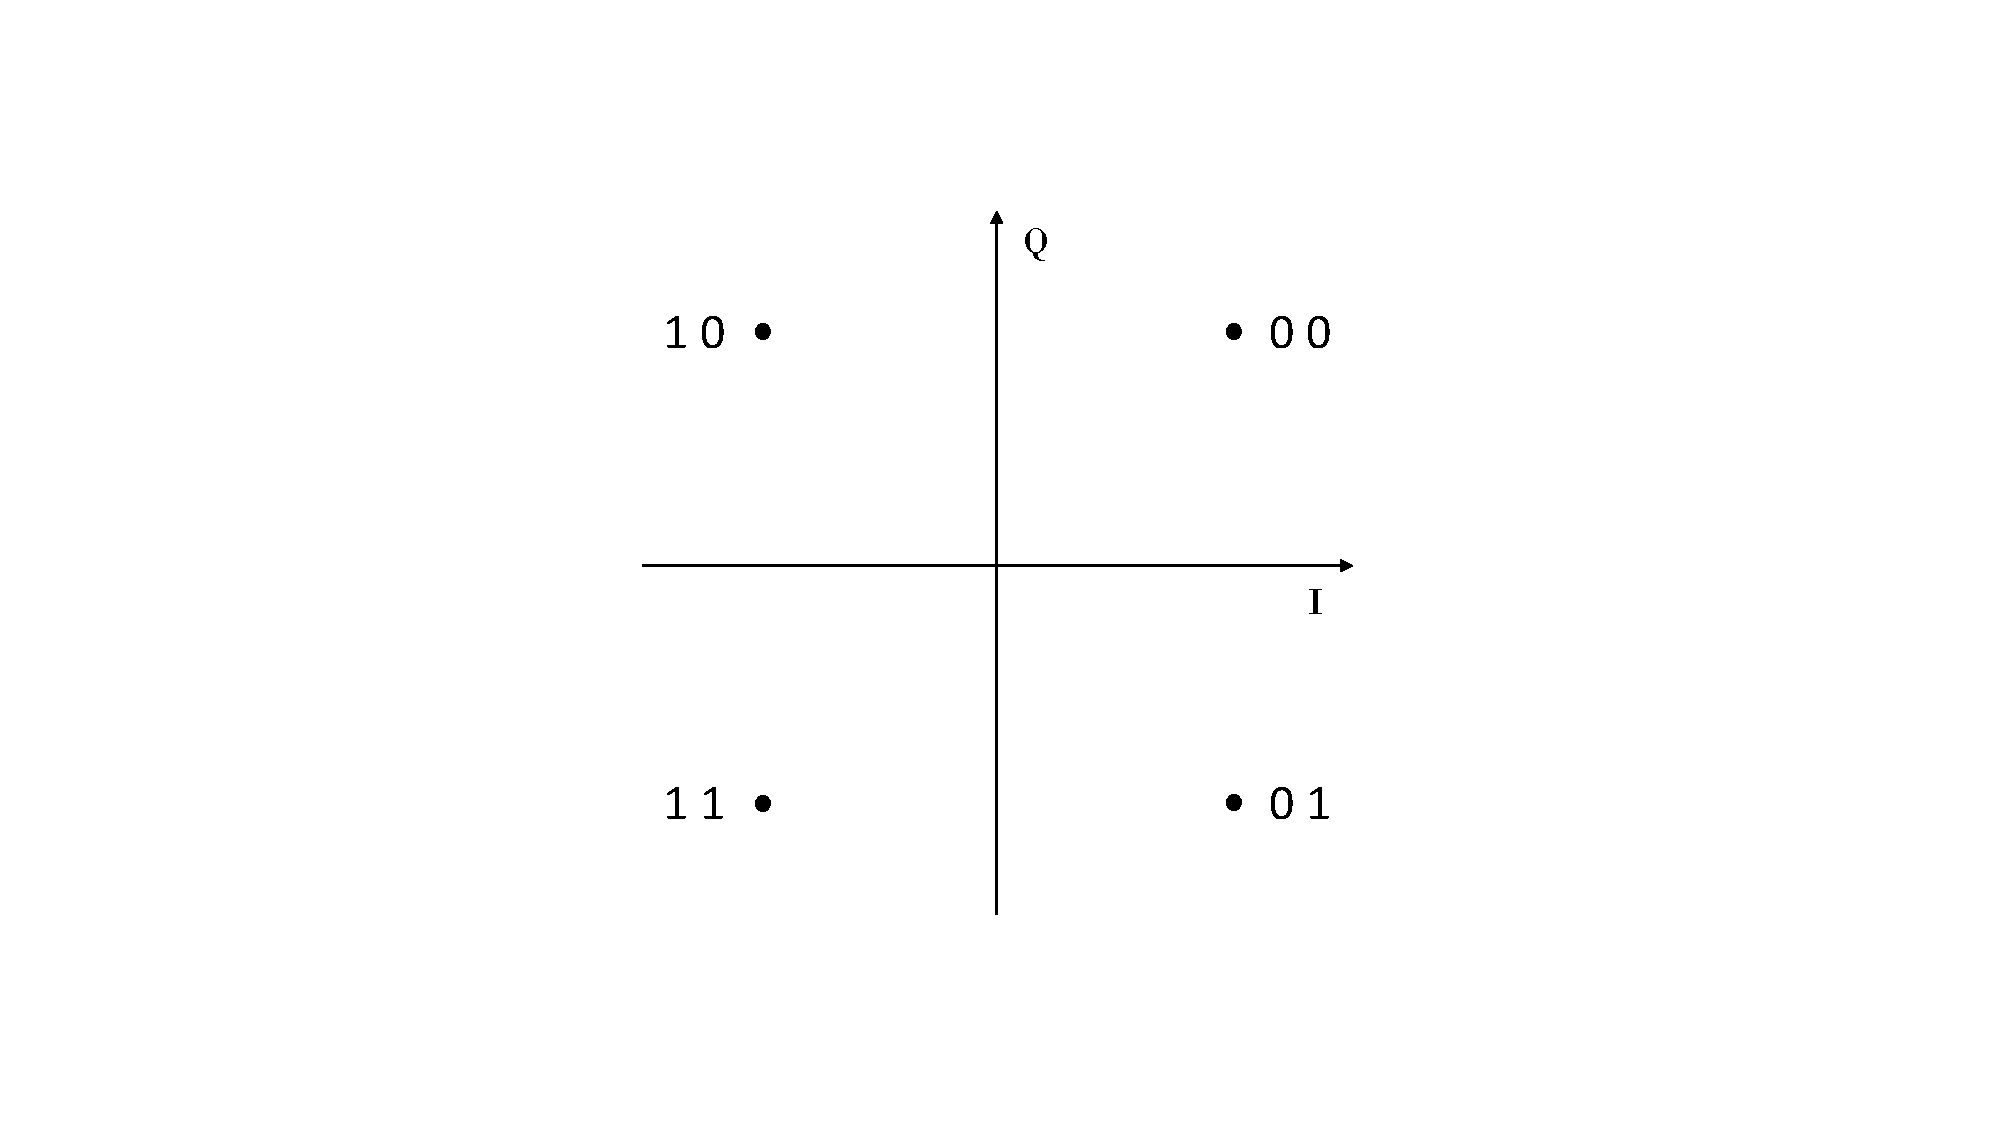
\includegraphics[width=0.6\textwidth]{./lib/m_qam_mapper/figures/MQAM_constellation}
	
	\caption{Constellation used to map the signal for m=4 }\label{constellation}
	
\end{figure}

\subsection*{Input Signals}

\subparagraph*{Number}: 1

\subparagraph*{Type}: Binary (DiscreteTimeDiscreteAmplitude)

\subsection*{Output Signals}

\subparagraph*{Number}: 2

\subparagraph*{Type}: Sequence of 1's and -1's (DiscreteTimeDiscreteAmplitude)

\subsection*{Example}

\begin{figure}
	\centering
	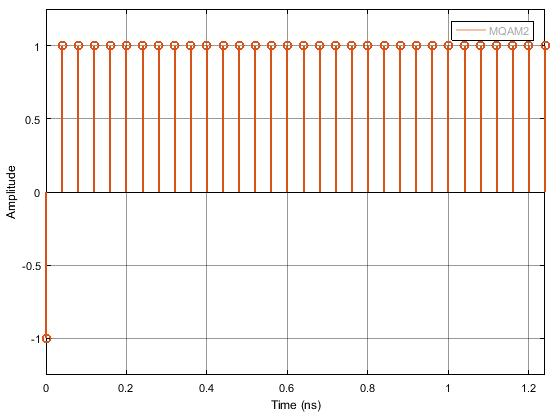
\includegraphics[width=\textwidth]{./lib/m_qam_mapper/figures/IQmodulator_output}
	
	\caption{Example of the type of signal generated by this block for the initial binary signal 0100... }\label{DeterministicAppendZeros}

\end{figure}

%\subsection*{Sugestions for future improvement}
